\documentclass[tikz,border=15pt,convert={outfile=rnnfwd.svg, command=\unexpanded{pdf2svg \infile\space\outfile}}]{standalone} % pdflatex --shell-escape rnnfwd.tex 
\usepackage{amsmath}
\usepackage{amssymb}
\renewcommand{\familydefault}{\sfdefault}

\usetikzlibrary{positioning, arrows.meta, shapes.geometric, calc}

\begin{document}
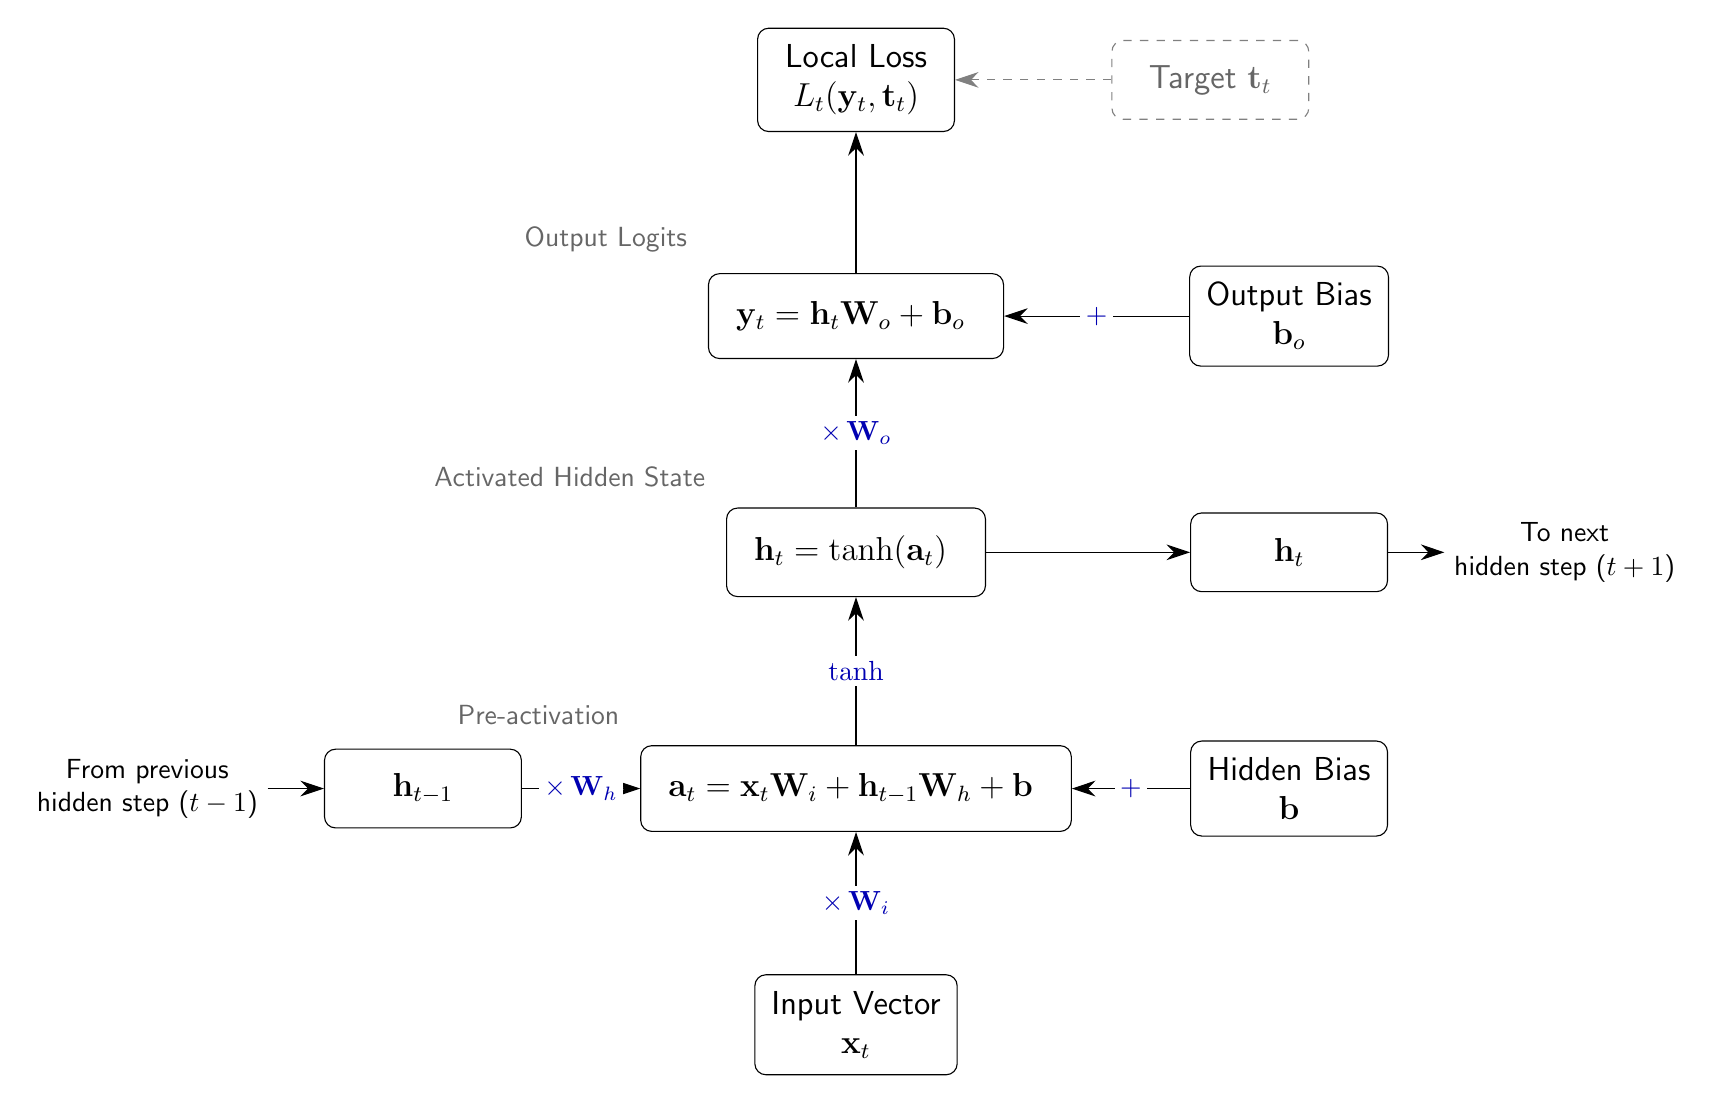
\begin{tikzpicture}[
    >={Stealth[length=3mm, width=2mm]},
    box/.style={draw, rounded corners, minimum width=2.5cm, minimum height=1cm, align=center, fill=white, font=\large, inner sep=6pt},
    txt/.style={align=center, font=\normalsize},
    edge_label/.style={fill=white, font=\normalsize, text=blue!70!black, inner sep=2pt}
]

% ================= Nodes =================

% Top level: Loss Calculation
\node[box] (loss) at (0, 7.5) {Local Loss \\ $L_t(\mathbf{y}_t, \mathbf{t}_t)$};
\node[box, draw=gray, dashed, text=gray!80!black] (target) at (4.5, 7.5) {Target $\mathbf{t}_t$};

% Output layer: Logits
\node[box, inner sep=10pt] (yt) at (0, 4.5) {
    $\displaystyle \mathbf{y}_t = \mathbf{h}_t \mathbf{W}_o + \mathbf{b}_o$
};
\node[box] (bias_o) at (5.5, 4.5) {Output Bias \\ $\mathbf{b}_o$};

% Central level: The explicit hidden state
\node[box, inner sep=10pt] (ht) at (0, 1.5) {
    $\displaystyle \mathbf{h}_t = \tanh(\mathbf{a}_t)$
};

% Lower Central: The pre-activation linear combination
\node[box, inner sep=10pt] (at) at (0, -1.5) {
    $\displaystyle \mathbf{a}_t = \mathbf{x}_t \mathbf{W}_i + \mathbf{h}_{t-1} \mathbf{W}_h + \mathbf{b}$
};

% Horizontal temporal flow (Left side: from past)
\node[txt] (prev_step_txt) at (-9, -1.5) {From previous \\ hidden step ($t-1$)};
\node[box] (from_prev) at (-5.5, -1.5) {$\mathbf{h}_{t-1}$};

% Horizontal temporal flow (Right side: to future)
\node[box] (to_next) at (5.5, 1.5) {$\mathbf{h}_t$};
\node[txt] (next_step_txt) at (9, 1.5) {To next \\ hidden step ($t+1$)};

% Bottom level: Inputs and parameters
\node[box] (xt) at (0, -4.5) {Input Vector \\ $\mathbf{x}_t$};
\node[box] (bias_h) at (5.5, -1.5) {Hidden Bias \\ $\mathbf{b}$};

% ================= Labels =================

\node[above left=0.2cm of yt, text=gray!80!black, font=\normalsize] {Output Logits};
\node[above left=0.2cm of ht, text=gray!80!black, font=\normalsize] {Activated Hidden State};
\node[above left=0.2cm of at, text=gray!80!black, font=\normalsize] {Pre-activation};

% ================= Edges =================

% Input to pre-activation
\draw[->] (xt) -- (at) node[midway, edge_label] {$\times \, \mathbf{W}_i$};

% Temporal connection from the past
\draw[->] (prev_step_txt) -- (from_prev);
\draw[->] (from_prev) -- (at) node[midway, edge_label] {$\times \, \mathbf{W}_h$};

% Hidden Bias addition
\draw[->] (bias_h) -- (at) node[midway, edge_label] {$+$};

% Pre-activation to hidden state
\draw[->] (at) -- (ht) node[midway, edge_label] {$\tanh$};

% Temporal connection to the future
\draw[->] (ht) -- (to_next);
\draw[->] (to_next) -- (next_step_txt);

% Hidden state to logits
\draw[->] (ht) -- (yt) node[midway, edge_label] {$\times \, \mathbf{W}_o$};

% Output Bias addition
\draw[->] (bias_o) -- (yt) node[midway, edge_label] {$+$};

% Logits and Target to Loss
\draw[->] (yt) -- (loss);
\draw[->, dashed, draw=gray] (target) -- (loss);

\end{tikzpicture}
\end{document}